
% Default to the notebook output style

    


% Inherit from the specified cell style.




    
\documentclass[11pt]{article}

    
    
    \usepackage[T1]{fontenc}
    % Nicer default font (+ math font) than Computer Modern for most use cases
    \usepackage{mathpazo}

    % Basic figure setup, for now with no caption control since it's done
    % automatically by Pandoc (which extracts ![](path) syntax from Markdown).
    \usepackage{graphicx}
    % We will generate all images so they have a width \maxwidth. This means
    % that they will get their normal width if they fit onto the page, but
    % are scaled down if they would overflow the margins.
    \makeatletter
    \def\maxwidth{\ifdim\Gin@nat@width>\linewidth\linewidth
    \else\Gin@nat@width\fi}
    \makeatother
    \let\Oldincludegraphics\includegraphics
    % Set max figure width to be 80% of text width, for now hardcoded.
    \renewcommand{\includegraphics}[1]{\Oldincludegraphics[width=.8\maxwidth]{#1}}
    % Ensure that by default, figures have no caption (until we provide a
    % proper Figure object with a Caption API and a way to capture that
    % in the conversion process - todo).
    \usepackage{caption}
    \DeclareCaptionLabelFormat{nolabel}{}
    \captionsetup{labelformat=nolabel}

    \usepackage{adjustbox} % Used to constrain images to a maximum size 
    \usepackage{xcolor} % Allow colors to be defined
    \usepackage{enumerate} % Needed for markdown enumerations to work
    \usepackage{geometry} % Used to adjust the document margins
    \usepackage{amsmath} % Equations
    \usepackage{amssymb} % Equations
    \usepackage{textcomp} % defines textquotesingle
    % Hack from http://tex.stackexchange.com/a/47451/13684:
    \AtBeginDocument{%
        \def\PYZsq{\textquotesingle}% Upright quotes in Pygmentized code
    }
    \usepackage{upquote} % Upright quotes for verbatim code
    \usepackage{eurosym} % defines \euro
    \usepackage[mathletters]{ucs} % Extended unicode (utf-8) support
    \usepackage[utf8x]{inputenc} % Allow utf-8 characters in the tex document
    \usepackage{fancyvrb} % verbatim replacement that allows latex
    \usepackage{grffile} % extends the file name processing of package graphics 
                         % to support a larger range 
    % The hyperref package gives us a pdf with properly built
    % internal navigation ('pdf bookmarks' for the table of contents,
    % internal cross-reference links, web links for URLs, etc.)
    \usepackage{hyperref}
    \usepackage{longtable} % longtable support required by pandoc >1.10
    \usepackage{booktabs}  % table support for pandoc > 1.12.2
    \usepackage[inline]{enumitem} % IRkernel/repr support (it uses the enumerate* environment)
    \usepackage[normalem]{ulem} % ulem is needed to support strikethroughs (\sout)
                                % normalem makes italics be italics, not underlines
    

    
    
    % Colors for the hyperref package
    \definecolor{urlcolor}{rgb}{0,.145,.698}
    \definecolor{linkcolor}{rgb}{.71,0.21,0.01}
    \definecolor{citecolor}{rgb}{.12,.54,.11}

    % ANSI colors
    \definecolor{ansi-black}{HTML}{3E424D}
    \definecolor{ansi-black-intense}{HTML}{282C36}
    \definecolor{ansi-red}{HTML}{E75C58}
    \definecolor{ansi-red-intense}{HTML}{B22B31}
    \definecolor{ansi-green}{HTML}{00A250}
    \definecolor{ansi-green-intense}{HTML}{007427}
    \definecolor{ansi-yellow}{HTML}{DDB62B}
    \definecolor{ansi-yellow-intense}{HTML}{B27D12}
    \definecolor{ansi-blue}{HTML}{208FFB}
    \definecolor{ansi-blue-intense}{HTML}{0065CA}
    \definecolor{ansi-magenta}{HTML}{D160C4}
    \definecolor{ansi-magenta-intense}{HTML}{A03196}
    \definecolor{ansi-cyan}{HTML}{60C6C8}
    \definecolor{ansi-cyan-intense}{HTML}{258F8F}
    \definecolor{ansi-white}{HTML}{C5C1B4}
    \definecolor{ansi-white-intense}{HTML}{A1A6B2}

    % commands and environments needed by pandoc snippets
    % extracted from the output of `pandoc -s`
    \providecommand{\tightlist}{%
      \setlength{\itemsep}{0pt}\setlength{\parskip}{0pt}}
    \DefineVerbatimEnvironment{Highlighting}{Verbatim}{commandchars=\\\{\}}
    % Add ',fontsize=\small' for more characters per line
    \newenvironment{Shaded}{}{}
    \newcommand{\KeywordTok}[1]{\textcolor[rgb]{0.00,0.44,0.13}{\textbf{{#1}}}}
    \newcommand{\DataTypeTok}[1]{\textcolor[rgb]{0.56,0.13,0.00}{{#1}}}
    \newcommand{\DecValTok}[1]{\textcolor[rgb]{0.25,0.63,0.44}{{#1}}}
    \newcommand{\BaseNTok}[1]{\textcolor[rgb]{0.25,0.63,0.44}{{#1}}}
    \newcommand{\FloatTok}[1]{\textcolor[rgb]{0.25,0.63,0.44}{{#1}}}
    \newcommand{\CharTok}[1]{\textcolor[rgb]{0.25,0.44,0.63}{{#1}}}
    \newcommand{\StringTok}[1]{\textcolor[rgb]{0.25,0.44,0.63}{{#1}}}
    \newcommand{\CommentTok}[1]{\textcolor[rgb]{0.38,0.63,0.69}{\textit{{#1}}}}
    \newcommand{\OtherTok}[1]{\textcolor[rgb]{0.00,0.44,0.13}{{#1}}}
    \newcommand{\AlertTok}[1]{\textcolor[rgb]{1.00,0.00,0.00}{\textbf{{#1}}}}
    \newcommand{\FunctionTok}[1]{\textcolor[rgb]{0.02,0.16,0.49}{{#1}}}
    \newcommand{\RegionMarkerTok}[1]{{#1}}
    \newcommand{\ErrorTok}[1]{\textcolor[rgb]{1.00,0.00,0.00}{\textbf{{#1}}}}
    \newcommand{\NormalTok}[1]{{#1}}
    
    % Additional commands for more recent versions of Pandoc
    \newcommand{\ConstantTok}[1]{\textcolor[rgb]{0.53,0.00,0.00}{{#1}}}
    \newcommand{\SpecialCharTok}[1]{\textcolor[rgb]{0.25,0.44,0.63}{{#1}}}
    \newcommand{\VerbatimStringTok}[1]{\textcolor[rgb]{0.25,0.44,0.63}{{#1}}}
    \newcommand{\SpecialStringTok}[1]{\textcolor[rgb]{0.73,0.40,0.53}{{#1}}}
    \newcommand{\ImportTok}[1]{{#1}}
    \newcommand{\DocumentationTok}[1]{\textcolor[rgb]{0.73,0.13,0.13}{\textit{{#1}}}}
    \newcommand{\AnnotationTok}[1]{\textcolor[rgb]{0.38,0.63,0.69}{\textbf{\textit{{#1}}}}}
    \newcommand{\CommentVarTok}[1]{\textcolor[rgb]{0.38,0.63,0.69}{\textbf{\textit{{#1}}}}}
    \newcommand{\VariableTok}[1]{\textcolor[rgb]{0.10,0.09,0.49}{{#1}}}
    \newcommand{\ControlFlowTok}[1]{\textcolor[rgb]{0.00,0.44,0.13}{\textbf{{#1}}}}
    \newcommand{\OperatorTok}[1]{\textcolor[rgb]{0.40,0.40,0.40}{{#1}}}
    \newcommand{\BuiltInTok}[1]{{#1}}
    \newcommand{\ExtensionTok}[1]{{#1}}
    \newcommand{\PreprocessorTok}[1]{\textcolor[rgb]{0.74,0.48,0.00}{{#1}}}
    \newcommand{\AttributeTok}[1]{\textcolor[rgb]{0.49,0.56,0.16}{{#1}}}
    \newcommand{\InformationTok}[1]{\textcolor[rgb]{0.38,0.63,0.69}{\textbf{\textit{{#1}}}}}
    \newcommand{\WarningTok}[1]{\textcolor[rgb]{0.38,0.63,0.69}{\textbf{\textit{{#1}}}}}
    
    
    % Define a nice break command that doesn't care if a line doesn't already
    % exist.
    \def\br{\hspace*{\fill} \\* }
    % Math Jax compatability definitions
    \def\gt{>}
    \def\lt{<}
    % Document parameters
    \title{Yapay Sinir A?lar?}
    
    
    

    % Pygments definitions
    
\makeatletter
\def\PY@reset{\let\PY@it=\relax \let\PY@bf=\relax%
    \let\PY@ul=\relax \let\PY@tc=\relax%
    \let\PY@bc=\relax \let\PY@ff=\relax}
\def\PY@tok#1{\csname PY@tok@#1\endcsname}
\def\PY@toks#1+{\ifx\relax#1\empty\else%
    \PY@tok{#1}\expandafter\PY@toks\fi}
\def\PY@do#1{\PY@bc{\PY@tc{\PY@ul{%
    \PY@it{\PY@bf{\PY@ff{#1}}}}}}}
\def\PY#1#2{\PY@reset\PY@toks#1+\relax+\PY@do{#2}}

\expandafter\def\csname PY@tok@w\endcsname{\def\PY@tc##1{\textcolor[rgb]{0.73,0.73,0.73}{##1}}}
\expandafter\def\csname PY@tok@c\endcsname{\let\PY@it=\textit\def\PY@tc##1{\textcolor[rgb]{0.25,0.50,0.50}{##1}}}
\expandafter\def\csname PY@tok@cp\endcsname{\def\PY@tc##1{\textcolor[rgb]{0.74,0.48,0.00}{##1}}}
\expandafter\def\csname PY@tok@k\endcsname{\let\PY@bf=\textbf\def\PY@tc##1{\textcolor[rgb]{0.00,0.50,0.00}{##1}}}
\expandafter\def\csname PY@tok@kp\endcsname{\def\PY@tc##1{\textcolor[rgb]{0.00,0.50,0.00}{##1}}}
\expandafter\def\csname PY@tok@kt\endcsname{\def\PY@tc##1{\textcolor[rgb]{0.69,0.00,0.25}{##1}}}
\expandafter\def\csname PY@tok@o\endcsname{\def\PY@tc##1{\textcolor[rgb]{0.40,0.40,0.40}{##1}}}
\expandafter\def\csname PY@tok@ow\endcsname{\let\PY@bf=\textbf\def\PY@tc##1{\textcolor[rgb]{0.67,0.13,1.00}{##1}}}
\expandafter\def\csname PY@tok@nb\endcsname{\def\PY@tc##1{\textcolor[rgb]{0.00,0.50,0.00}{##1}}}
\expandafter\def\csname PY@tok@nf\endcsname{\def\PY@tc##1{\textcolor[rgb]{0.00,0.00,1.00}{##1}}}
\expandafter\def\csname PY@tok@nc\endcsname{\let\PY@bf=\textbf\def\PY@tc##1{\textcolor[rgb]{0.00,0.00,1.00}{##1}}}
\expandafter\def\csname PY@tok@nn\endcsname{\let\PY@bf=\textbf\def\PY@tc##1{\textcolor[rgb]{0.00,0.00,1.00}{##1}}}
\expandafter\def\csname PY@tok@ne\endcsname{\let\PY@bf=\textbf\def\PY@tc##1{\textcolor[rgb]{0.82,0.25,0.23}{##1}}}
\expandafter\def\csname PY@tok@nv\endcsname{\def\PY@tc##1{\textcolor[rgb]{0.10,0.09,0.49}{##1}}}
\expandafter\def\csname PY@tok@no\endcsname{\def\PY@tc##1{\textcolor[rgb]{0.53,0.00,0.00}{##1}}}
\expandafter\def\csname PY@tok@nl\endcsname{\def\PY@tc##1{\textcolor[rgb]{0.63,0.63,0.00}{##1}}}
\expandafter\def\csname PY@tok@ni\endcsname{\let\PY@bf=\textbf\def\PY@tc##1{\textcolor[rgb]{0.60,0.60,0.60}{##1}}}
\expandafter\def\csname PY@tok@na\endcsname{\def\PY@tc##1{\textcolor[rgb]{0.49,0.56,0.16}{##1}}}
\expandafter\def\csname PY@tok@nt\endcsname{\let\PY@bf=\textbf\def\PY@tc##1{\textcolor[rgb]{0.00,0.50,0.00}{##1}}}
\expandafter\def\csname PY@tok@nd\endcsname{\def\PY@tc##1{\textcolor[rgb]{0.67,0.13,1.00}{##1}}}
\expandafter\def\csname PY@tok@s\endcsname{\def\PY@tc##1{\textcolor[rgb]{0.73,0.13,0.13}{##1}}}
\expandafter\def\csname PY@tok@sd\endcsname{\let\PY@it=\textit\def\PY@tc##1{\textcolor[rgb]{0.73,0.13,0.13}{##1}}}
\expandafter\def\csname PY@tok@si\endcsname{\let\PY@bf=\textbf\def\PY@tc##1{\textcolor[rgb]{0.73,0.40,0.53}{##1}}}
\expandafter\def\csname PY@tok@se\endcsname{\let\PY@bf=\textbf\def\PY@tc##1{\textcolor[rgb]{0.73,0.40,0.13}{##1}}}
\expandafter\def\csname PY@tok@sr\endcsname{\def\PY@tc##1{\textcolor[rgb]{0.73,0.40,0.53}{##1}}}
\expandafter\def\csname PY@tok@ss\endcsname{\def\PY@tc##1{\textcolor[rgb]{0.10,0.09,0.49}{##1}}}
\expandafter\def\csname PY@tok@sx\endcsname{\def\PY@tc##1{\textcolor[rgb]{0.00,0.50,0.00}{##1}}}
\expandafter\def\csname PY@tok@m\endcsname{\def\PY@tc##1{\textcolor[rgb]{0.40,0.40,0.40}{##1}}}
\expandafter\def\csname PY@tok@gh\endcsname{\let\PY@bf=\textbf\def\PY@tc##1{\textcolor[rgb]{0.00,0.00,0.50}{##1}}}
\expandafter\def\csname PY@tok@gu\endcsname{\let\PY@bf=\textbf\def\PY@tc##1{\textcolor[rgb]{0.50,0.00,0.50}{##1}}}
\expandafter\def\csname PY@tok@gd\endcsname{\def\PY@tc##1{\textcolor[rgb]{0.63,0.00,0.00}{##1}}}
\expandafter\def\csname PY@tok@gi\endcsname{\def\PY@tc##1{\textcolor[rgb]{0.00,0.63,0.00}{##1}}}
\expandafter\def\csname PY@tok@gr\endcsname{\def\PY@tc##1{\textcolor[rgb]{1.00,0.00,0.00}{##1}}}
\expandafter\def\csname PY@tok@ge\endcsname{\let\PY@it=\textit}
\expandafter\def\csname PY@tok@gs\endcsname{\let\PY@bf=\textbf}
\expandafter\def\csname PY@tok@gp\endcsname{\let\PY@bf=\textbf\def\PY@tc##1{\textcolor[rgb]{0.00,0.00,0.50}{##1}}}
\expandafter\def\csname PY@tok@go\endcsname{\def\PY@tc##1{\textcolor[rgb]{0.53,0.53,0.53}{##1}}}
\expandafter\def\csname PY@tok@gt\endcsname{\def\PY@tc##1{\textcolor[rgb]{0.00,0.27,0.87}{##1}}}
\expandafter\def\csname PY@tok@err\endcsname{\def\PY@bc##1{\setlength{\fboxsep}{0pt}\fcolorbox[rgb]{1.00,0.00,0.00}{1,1,1}{\strut ##1}}}
\expandafter\def\csname PY@tok@kc\endcsname{\let\PY@bf=\textbf\def\PY@tc##1{\textcolor[rgb]{0.00,0.50,0.00}{##1}}}
\expandafter\def\csname PY@tok@kd\endcsname{\let\PY@bf=\textbf\def\PY@tc##1{\textcolor[rgb]{0.00,0.50,0.00}{##1}}}
\expandafter\def\csname PY@tok@kn\endcsname{\let\PY@bf=\textbf\def\PY@tc##1{\textcolor[rgb]{0.00,0.50,0.00}{##1}}}
\expandafter\def\csname PY@tok@kr\endcsname{\let\PY@bf=\textbf\def\PY@tc##1{\textcolor[rgb]{0.00,0.50,0.00}{##1}}}
\expandafter\def\csname PY@tok@bp\endcsname{\def\PY@tc##1{\textcolor[rgb]{0.00,0.50,0.00}{##1}}}
\expandafter\def\csname PY@tok@fm\endcsname{\def\PY@tc##1{\textcolor[rgb]{0.00,0.00,1.00}{##1}}}
\expandafter\def\csname PY@tok@vc\endcsname{\def\PY@tc##1{\textcolor[rgb]{0.10,0.09,0.49}{##1}}}
\expandafter\def\csname PY@tok@vg\endcsname{\def\PY@tc##1{\textcolor[rgb]{0.10,0.09,0.49}{##1}}}
\expandafter\def\csname PY@tok@vi\endcsname{\def\PY@tc##1{\textcolor[rgb]{0.10,0.09,0.49}{##1}}}
\expandafter\def\csname PY@tok@vm\endcsname{\def\PY@tc##1{\textcolor[rgb]{0.10,0.09,0.49}{##1}}}
\expandafter\def\csname PY@tok@sa\endcsname{\def\PY@tc##1{\textcolor[rgb]{0.73,0.13,0.13}{##1}}}
\expandafter\def\csname PY@tok@sb\endcsname{\def\PY@tc##1{\textcolor[rgb]{0.73,0.13,0.13}{##1}}}
\expandafter\def\csname PY@tok@sc\endcsname{\def\PY@tc##1{\textcolor[rgb]{0.73,0.13,0.13}{##1}}}
\expandafter\def\csname PY@tok@dl\endcsname{\def\PY@tc##1{\textcolor[rgb]{0.73,0.13,0.13}{##1}}}
\expandafter\def\csname PY@tok@s2\endcsname{\def\PY@tc##1{\textcolor[rgb]{0.73,0.13,0.13}{##1}}}
\expandafter\def\csname PY@tok@sh\endcsname{\def\PY@tc##1{\textcolor[rgb]{0.73,0.13,0.13}{##1}}}
\expandafter\def\csname PY@tok@s1\endcsname{\def\PY@tc##1{\textcolor[rgb]{0.73,0.13,0.13}{##1}}}
\expandafter\def\csname PY@tok@mb\endcsname{\def\PY@tc##1{\textcolor[rgb]{0.40,0.40,0.40}{##1}}}
\expandafter\def\csname PY@tok@mf\endcsname{\def\PY@tc##1{\textcolor[rgb]{0.40,0.40,0.40}{##1}}}
\expandafter\def\csname PY@tok@mh\endcsname{\def\PY@tc##1{\textcolor[rgb]{0.40,0.40,0.40}{##1}}}
\expandafter\def\csname PY@tok@mi\endcsname{\def\PY@tc##1{\textcolor[rgb]{0.40,0.40,0.40}{##1}}}
\expandafter\def\csname PY@tok@il\endcsname{\def\PY@tc##1{\textcolor[rgb]{0.40,0.40,0.40}{##1}}}
\expandafter\def\csname PY@tok@mo\endcsname{\def\PY@tc##1{\textcolor[rgb]{0.40,0.40,0.40}{##1}}}
\expandafter\def\csname PY@tok@ch\endcsname{\let\PY@it=\textit\def\PY@tc##1{\textcolor[rgb]{0.25,0.50,0.50}{##1}}}
\expandafter\def\csname PY@tok@cm\endcsname{\let\PY@it=\textit\def\PY@tc##1{\textcolor[rgb]{0.25,0.50,0.50}{##1}}}
\expandafter\def\csname PY@tok@cpf\endcsname{\let\PY@it=\textit\def\PY@tc##1{\textcolor[rgb]{0.25,0.50,0.50}{##1}}}
\expandafter\def\csname PY@tok@c1\endcsname{\let\PY@it=\textit\def\PY@tc##1{\textcolor[rgb]{0.25,0.50,0.50}{##1}}}
\expandafter\def\csname PY@tok@cs\endcsname{\let\PY@it=\textit\def\PY@tc##1{\textcolor[rgb]{0.25,0.50,0.50}{##1}}}

\def\PYZbs{\char`\\}
\def\PYZus{\char`\_}
\def\PYZob{\char`\{}
\def\PYZcb{\char`\}}
\def\PYZca{\char`\^}
\def\PYZam{\char`\&}
\def\PYZlt{\char`\<}
\def\PYZgt{\char`\>}
\def\PYZsh{\char`\#}
\def\PYZpc{\char`\%}
\def\PYZdl{\char`\$}
\def\PYZhy{\char`\-}
\def\PYZsq{\char`\'}
\def\PYZdq{\char`\"}
\def\PYZti{\char`\~}
% for compatibility with earlier versions
\def\PYZat{@}
\def\PYZlb{[}
\def\PYZrb{]}
\makeatother


    % Exact colors from NB
    \definecolor{incolor}{rgb}{0.0, 0.0, 0.5}
    \definecolor{outcolor}{rgb}{0.545, 0.0, 0.0}



    
    % Prevent overflowing lines due to hard-to-break entities
    \sloppy 
    % Setup hyperref package
    \hypersetup{
      breaklinks=true,  % so long urls are correctly broken across lines
      colorlinks=true,
      urlcolor=urlcolor,
      linkcolor=linkcolor,
      citecolor=citecolor,
      }
    % Slightly bigger margins than the latex defaults
    
    \geometry{verbose,tmargin=1in,bmargin=1in,lmargin=1in,rmargin=1in}
    
    

    \begin{document}
    
    
    \maketitle
    
    

    
    \section{Yapay Sinir Ağları}\label{yapay-sinir-aux11flarux131}

\begin{figure}
\centering
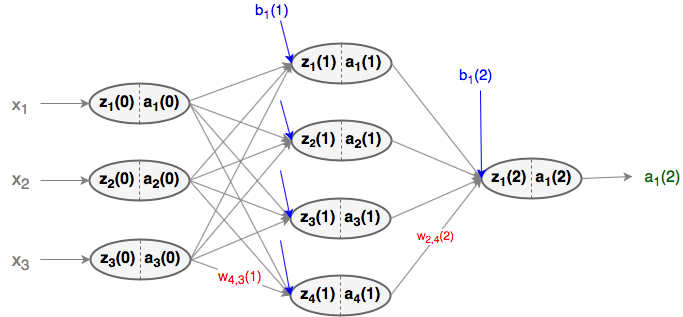
\includegraphics{network.png}
\caption{}
\end{figure}

\subsection{İleri Besleme}\label{ileri-besleme}

\begin{itemize}
\tightlist
\item
  \$ Z(t) = W(t)A(t-1) + b(t) \$
\item
  \$ A(t) = \sigma(Z(t)) \$
\end{itemize}

\[
Z(t) = 
\begin{bmatrix}
. \\
z_2(t) \\
. \\
. \\
\end{bmatrix}
=
\begin{bmatrix}
.       & . & . \\
 w_{i1}(t)       & w_{i2}(t)  & w_{i3}(t)  \\
.       & . & . \\
.       & . & . \\
\end{bmatrix}
\begin{bmatrix}
a_1(t-1) \\
a_2(t-1)\\
a_3(t-1)\\
\end{bmatrix}
+
\begin{bmatrix}
. \\
b_2(t) \\
. \\
. \\
\end{bmatrix}
\]

\paragraph{Yardımcı Türevler}\label{yardux131mcux131-tuxfcrevler}

\[
\frac{dz_i(t)}{ dw_{ij}(t)} = a_j(t-1)
\;\;\;\text{   ve   }\;\;\;
\frac{dz_i(t)}{db_{i}(t)} = 1
\] ayrıca

\[
\frac{dz_i(t)}{dz_j(t-1)} = 
\frac{dz_i(t)}{da_j(t-1)} \frac{da_j(t-1)}{dz_j(t-1)} =  
w_{ij}(t) \sigma'(z_j(t-1)) 
\]

\subsection{Geri Besleme}\label{geri-besleme}

\paragraph{Odak}\label{odak}

\[
\triangle_i(t) =
\frac{dH}{ dz_{i}(t)} 
\] \#\#\#\# Aranılan Türevler \[
\frac{dH}{ dw_{ij}(t)} = 
\frac{dH}{ dz_i(t)}
\frac{dz_i(t)}{ dw_{ij}(t)} =
\triangle_i(t) a_j(t-1)
\] ve \[
\frac{dH}{ db_{i}(t)} 
=\frac{dH}{ dz_i(t)}
\frac{dz_i(t)}{ db_{i}(t)} 
= \triangle_i(t)
\]

\paragraph{Geri yayılım}\label{geri-yayux131lux131m}

\begin{figure}
\centering
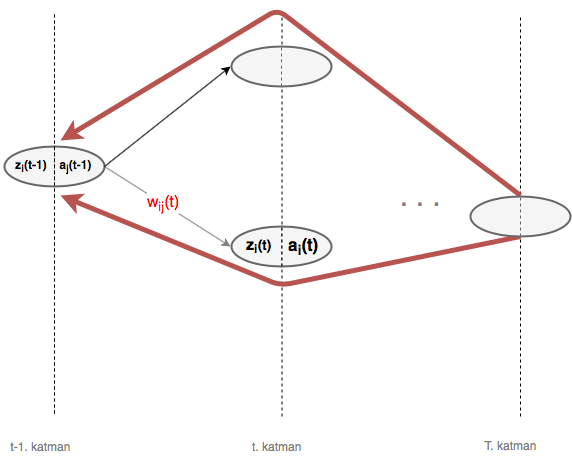
\includegraphics{geriyayilim.png}
\caption{}
\end{figure}

\(t.\) katmandaki bütün \(\triangle_i(t)\) biliniyorsa, bir önceki
katmandaki \(\triangle_j(t-1)\) nasıl hesaplanır?

\[
\triangle_j(t-1) =
\frac{dH}{ dz_{j}(t-1)} 
= \sum_i \frac{dH}{ dz_{i}(t)} \frac{dz_i(t)}{dz_j(t-1)}
= \sum_i \triangle_i(t) w_{ij}(t) \sigma'(z_j(t-1)) 
\]

Dolayısıyla \[
\triangle(t-1) 
= W^T(t) \triangle(t)  * \sigma'(z_j(t-1)) 
\]

    \section{Geri yayılım
Algoritması}\label{geri-yayux131lux131m-algoritmasux131}

\paragraph{Gradyan iniş}\label{gradyan-iniux15f}

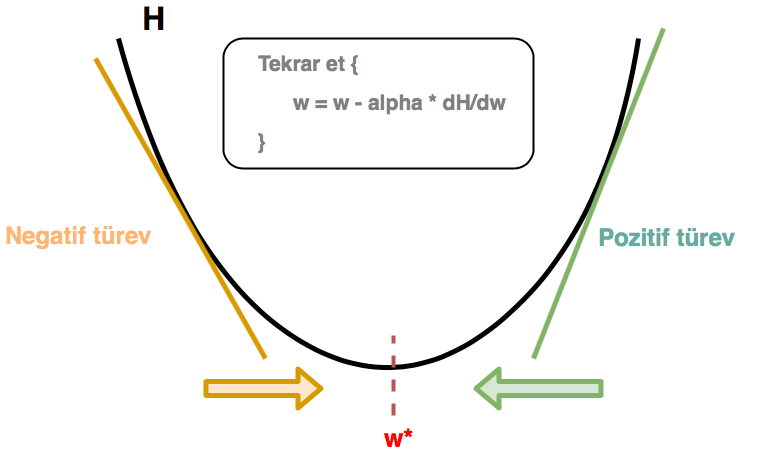
\includegraphics{gradyan.png} \#\#\# Hata \[
H = \frac{1}{2n} \sum^n_{i=1} (y_i - a_i(T))^2
\]

\subsubsection{Hatanın son katmana göre
türevi}\label{hatanux131n-son-katmana-guxf6re-tuxfcrevi}

\[
\triangle(T) =  \frac{dH}{ dz(T)} = \frac{dH}{ da(T)} \frac{da(T)}{ dz(T)}
= (a(T) - y) * \sigma'(z(T))
\]

\subsubsection{Hatanın geri
yayılımı}\label{hatanux131n-geri-yayux131lux131mux131}

\[
\triangle(t-1) 
= W^T(t) \triangle(t)  * \sigma'(z_j(t-1)) 
\]

\subsubsection{En iyi parametreleri
bulmak}\label{en-iyi-parametreleri-bulmak}

\[
\frac{dH}{ dw_{ij}(t)} = 
\triangle_i(t) a_j(t-1)
\] ve \[
\frac{dH}{ db_{i}(t)} 
= \triangle_i(t)
\]

\section{Görüntülerde duygu
tanıma}\label{guxf6ruxfcntuxfclerde-duygu-tanux131ma}

Burada öğrendiklerimizi ve yazdfığımız YSA kodunu şu veri seti üzerinde
deneyebilirsiniz.

https://www.kaggle.com/c/challenges-in-representation-learning-facial-expression-recognition-challenge

    \begin{Verbatim}[commandchars=\\\{\}]
{\color{incolor}In [{\color{incolor}1}]:} \PY{c+c1}{\PYZsh{} Importing the libraries}
        \PY{k+kn}{import} \PY{n+nn}{numpy} \PY{k}{as} \PY{n+nn}{np}
        \PY{k+kn}{import} \PY{n+nn}{matplotlib}\PY{n+nn}{.}\PY{n+nn}{pyplot} \PY{k}{as} \PY{n+nn}{plt}
        \PY{o}{\PYZpc{}}\PY{k}{matplotlib} inline  
        \PY{k+kn}{import} \PY{n+nn}{pandas} \PY{k}{as} \PY{n+nn}{pd}
        \PY{k+kn}{import} \PY{n+nn}{warnings}
        \PY{n}{warnings}\PY{o}{.}\PY{n}{filterwarnings}\PY{p}{(}\PY{l+s+s1}{\PYZsq{}}\PY{l+s+s1}{ignore}\PY{l+s+s1}{\PYZsq{}}\PY{p}{)}
        \PY{k+kn}{import} \PY{n+nn}{timeit}
        \PY{k+kn}{import} \PY{n+nn}{random}
\end{Verbatim}


    \begin{Verbatim}[commandchars=\\\{\}]
{\color{incolor}In [{\color{incolor}2}]:} \PY{k}{class} \PY{n+nc}{yapay\PYZus{}sinir\PYZus{}agi}\PY{p}{(}\PY{p}{)}\PY{p}{:}
            \PY{k}{def} \PY{n+nf}{\PYZus{}\PYZus{}init\PYZus{}\PYZus{}}\PY{p}{(}\PY{n+nb+bp}{self}\PY{p}{,} \PY{n}{katmanlar}\PY{p}{)}\PY{p}{:}
                \PY{n+nb+bp}{self}\PY{o}{.}\PY{n}{katmanlar} \PY{o}{=} \PY{n}{katmanlar}
                \PY{n+nb+bp}{self}\PY{o}{.}\PY{n}{b} \PY{o}{=} \PY{p}{[}\PY{n}{np}\PY{o}{.}\PY{n}{random}\PY{o}{.}\PY{n}{randn}\PY{p}{(}\PY{n}{k}\PY{p}{,} \PY{l+m+mi}{1}\PY{p}{)} \PY{k}{for} \PY{n}{k} \PY{o+ow}{in} \PY{n+nb+bp}{self}\PY{o}{.}\PY{n}{katmanlar}\PY{p}{[}\PY{l+m+mi}{1}\PY{p}{:}\PY{p}{]}\PY{p}{]} \PY{c+c1}{\PYZsh{} bias degerleri (ilk katman haric)}
                \PY{n+nb+bp}{self}\PY{o}{.}\PY{n}{W} \PY{o}{=} \PY{p}{[}\PY{n}{np}\PY{o}{.}\PY{n}{random}\PY{o}{.}\PY{n}{randn}\PY{p}{(}\PY{n}{k2}\PY{p}{,} \PY{n}{k1}\PY{p}{)} \PY{k}{for} \PY{n}{k1}\PY{p}{,} \PY{n}{k2} \PY{o+ow}{in} \PY{n+nb}{zip}\PY{p}{(}\PY{n+nb+bp}{self}\PY{o}{.}\PY{n}{katmanlar}\PY{p}{[}\PY{p}{:}\PY{o}{\PYZhy{}}\PY{l+m+mi}{1}\PY{p}{]}\PY{p}{,}\PY{n+nb+bp}{self}\PY{o}{.}\PY{n}{katmanlar}\PY{p}{[}\PY{l+m+mi}{1}\PY{p}{:}\PY{p}{]}\PY{p}{)}\PY{p}{]}
                \PY{n+nb+bp}{self}\PY{o}{.}\PY{n}{H} \PY{o}{=} \PY{p}{[}\PY{p}{]} \PY{c+c1}{\PYZsh{} hata}
                
                \PY{n+nb+bp}{self}\PY{o}{.}\PY{n}{onlyOnce} \PY{o}{=} \PY{k+kc}{True}
        
            \PY{k}{def} \PY{n+nf}{ag}\PY{p}{(}\PY{n+nb+bp}{self}\PY{p}{)}\PY{p}{:}
                \PY{k}{return} \PY{n+nb+bp}{self}\PY{o}{.}\PY{n}{W}\PY{p}{,} \PY{n+nb+bp}{self}\PY{o}{.}\PY{n}{b}
            
            \PY{k}{def} \PY{n+nf}{ileribesleme}\PY{p}{(}\PY{n+nb+bp}{self}\PY{p}{,} \PY{n}{a}\PY{p}{)}\PY{p}{:}
                \PY{l+s+sd}{\PYZdq{}\PYZdq{}\PYZdq{}Katman katman yeni a degerleri hesaplaniyor\PYZdq{}\PYZdq{}\PYZdq{}}
                \PY{n}{a} \PY{o}{=} \PY{n+nb+bp}{self}\PY{o}{.}\PY{n}{checkDimension}\PY{p}{(}\PY{n}{a}\PY{p}{)}
                \PY{k}{for} \PY{n}{w}\PY{p}{,} \PY{n}{b} \PY{o+ow}{in} \PY{n+nb}{zip}\PY{p}{(}\PY{n+nb+bp}{self}\PY{o}{.}\PY{n}{W}\PY{p}{,} \PY{n+nb+bp}{self}\PY{o}{.}\PY{n}{b}\PY{p}{)}\PY{p}{:}
                    \PY{n}{z} \PY{o}{=} \PY{n}{np}\PY{o}{.}\PY{n}{dot}\PY{p}{(}\PY{n}{w}\PY{p}{,} \PY{n}{a}\PY{p}{)}\PY{o}{+}\PY{n}{b}
                    \PY{n}{a} \PY{o}{=} \PY{n+nb+bp}{self}\PY{o}{.}\PY{n}{sigmoid}\PY{p}{(}\PY{n}{z}\PY{p}{)}
                \PY{k}{return} \PY{n}{a}
            
            \PY{k}{def} \PY{n+nf}{geribesleme}\PY{p}{(}\PY{n+nb+bp}{self}\PY{p}{,}\PY{n}{X}\PY{p}{,}\PY{n}{y}\PY{p}{)}\PY{p}{:}
                \PY{n}{delta\PYZus{}b} \PY{o}{=} \PY{p}{[}\PY{n}{np}\PY{o}{.}\PY{n}{zeros}\PY{p}{(}\PY{n}{b}\PY{o}{.}\PY{n}{shape}\PY{p}{)} \PY{k}{for} \PY{n}{b} \PY{o+ow}{in} \PY{n+nb+bp}{self}\PY{o}{.}\PY{n}{b}\PY{p}{]}
                \PY{n}{delta\PYZus{}w} \PY{o}{=} \PY{p}{[}\PY{n}{np}\PY{o}{.}\PY{n}{zeros}\PY{p}{(}\PY{n}{w}\PY{o}{.}\PY{n}{shape}\PY{p}{)} \PY{k}{for} \PY{n}{w} \PY{o+ow}{in} \PY{n+nb+bp}{self}\PY{o}{.}\PY{n}{W}\PY{p}{]}
                \PY{n}{a} \PY{o}{=} \PY{n}{X}\PY{p}{;} \PY{n}{A}\PY{p}{,} \PY{n}{Z} \PY{o}{=} \PY{p}{[}\PY{n}{a}\PY{p}{]}\PY{p}{,} \PY{p}{[}\PY{p}{]}  \PY{c+c1}{\PYZsh{} A, Z degerleri}
                \PY{k}{for} \PY{n}{w}\PY{p}{,} \PY{n}{b} \PY{o+ow}{in} \PY{n+nb}{zip}\PY{p}{(}\PY{n+nb+bp}{self}\PY{o}{.}\PY{n}{W}\PY{p}{,} \PY{n+nb+bp}{self}\PY{o}{.}\PY{n}{b}\PY{p}{)}\PY{p}{:}\PY{c+c1}{\PYZsh{} z ve a degerlerini depolayalim}
                    \PY{n}{z} \PY{o}{=} \PY{n}{np}\PY{o}{.}\PY{n}{dot}\PY{p}{(}\PY{n}{w}\PY{p}{,} \PY{n}{a}\PY{p}{)} \PY{o}{+} \PY{n}{b}
                    \PY{n}{a} \PY{o}{=} \PY{n+nb+bp}{self}\PY{o}{.}\PY{n}{sigmoid}\PY{p}{(}\PY{n}{z}\PY{p}{)}
                    \PY{n}{Z}\PY{o}{.}\PY{n}{append}\PY{p}{(}\PY{n}{z}\PY{p}{)}\PY{p}{;} \PY{n}{A}\PY{o}{.}\PY{n}{append}\PY{p}{(}\PY{n}{a}\PY{p}{)}
                    
                    \PY{n+nb+bp}{self}\PY{o}{.}\PY{n}{printShape}\PY{p}{(}\PY{n}{b}\PY{p}{,} \PY{l+s+s2}{\PYZdq{}}\PY{l+s+s2}{b}\PY{l+s+s2}{\PYZdq{}}\PY{p}{,} \PY{n}{w}\PY{p}{,} \PY{l+s+s2}{\PYZdq{}}\PY{l+s+s2}{w}\PY{l+s+s2}{\PYZdq{}}\PY{p}{)}
        
        
                
                \PY{n}{hata} \PY{o}{=} \PY{n}{A}\PY{p}{[}\PY{o}{\PYZhy{}}\PY{l+m+mi}{1}\PY{p}{]} \PY{o}{\PYZhy{}} \PY{n}{y} \PY{c+c1}{\PYZsh{} En son katmandaki hata }
                \PY{n}{delta} \PY{o}{=} \PY{n}{hata} \PY{o}{*} \PY{n+nb+bp}{self}\PY{o}{.}\PY{n}{sigmoid\PYZus{}turevi}\PY{p}{(}\PY{n}{Z}\PY{p}{[}\PY{o}{\PYZhy{}}\PY{l+m+mi}{1}\PY{p}{]}\PY{p}{)}
                \PY{n}{delta\PYZus{}b}\PY{p}{[}\PY{o}{\PYZhy{}}\PY{l+m+mi}{1}\PY{p}{]} \PY{o}{=} \PY{n}{delta} \PY{c+c1}{\PYZsh{} Son katmanda W, b\PYZsq{}deki degisim  }
                \PY{n}{delta\PYZus{}w}\PY{p}{[}\PY{o}{\PYZhy{}}\PY{l+m+mi}{1}\PY{p}{]} \PY{o}{=} \PY{n}{delta} \PY{o}{*} \PY{n}{A}\PY{p}{[}\PY{o}{\PYZhy{}}\PY{l+m+mi}{2}\PY{p}{]}\PY{o}{.}\PY{n}{T} \PY{c+c1}{\PYZsh{} ERROR: np.dot(delta, A[\PYZhy{}2].T)}
                
                \PY{n+nb+bp}{self}\PY{o}{.}\PY{n}{printShape}\PY{p}{(}\PY{n}{delta\PYZus{}b}\PY{p}{[}\PY{o}{\PYZhy{}}\PY{l+m+mi}{1}\PY{p}{]}\PY{p}{,} \PY{l+s+s2}{\PYZdq{}}\PY{l+s+s2}{delta\PYZus{}b[\PYZhy{}1]}\PY{l+s+s2}{\PYZdq{}}\PY{p}{,} \PY{n}{delta\PYZus{}w}\PY{p}{[}\PY{o}{\PYZhy{}}\PY{l+m+mi}{1}\PY{p}{]}\PY{p}{,} \PY{l+s+s2}{\PYZdq{}}\PY{l+s+s2}{delta\PYZus{}w[\PYZhy{}1]}\PY{l+s+s2}{\PYZdq{}}\PY{p}{)}
                
                \PY{k}{for} \PY{n}{k} \PY{o+ow}{in} \PY{n+nb}{range}\PY{p}{(}\PY{l+m+mi}{2}\PY{p}{,} \PY{n+nb}{len}\PY{p}{(}\PY{n+nb+bp}{self}\PY{o}{.}\PY{n}{katmanlar}\PY{p}{)}\PY{p}{)}\PY{p}{:} \PY{c+c1}{\PYZsh{} Hatanin geriye yayilimi}
                    \PY{n}{delta} \PY{o}{=} \PY{n}{np}\PY{o}{.}\PY{n}{dot}\PY{p}{(}\PY{n+nb+bp}{self}\PY{o}{.}\PY{n}{W}\PY{p}{[}\PY{o}{\PYZhy{}}\PY{n}{k}\PY{o}{+}\PY{l+m+mi}{1}\PY{p}{]}\PY{o}{.}\PY{n}{T}\PY{p}{,} \PY{n}{delta}\PY{p}{)} \PY{o}{*} \PY{n+nb+bp}{self}\PY{o}{.}\PY{n}{sigmoid\PYZus{}turevi}\PY{p}{(}\PY{n}{Z}\PY{p}{[}\PY{o}{\PYZhy{}}\PY{n}{k}\PY{p}{]}\PY{p}{)}
                    \PY{n}{delta\PYZus{}b}\PY{p}{[}\PY{o}{\PYZhy{}}\PY{n}{k}\PY{p}{]} \PY{o}{=} \PY{n}{delta}
                    \PY{n}{delta\PYZus{}w}\PY{p}{[}\PY{o}{\PYZhy{}}\PY{n}{k}\PY{p}{]} \PY{o}{=} \PY{n}{delta} \PY{o}{*} \PY{n}{A}\PY{p}{[}\PY{o}{\PYZhy{}}\PY{n}{k}\PY{o}{\PYZhy{}}\PY{l+m+mi}{1}\PY{p}{]}\PY{o}{.}\PY{n}{T} \PY{c+c1}{\PYZsh{} ERROR: np.dot(delta, A[\PYZhy{}k\PYZhy{}1].T)}
                    
                    \PY{n+nb+bp}{self}\PY{o}{.}\PY{n}{printShape}\PY{p}{(}\PY{n}{delta\PYZus{}b}\PY{p}{[}\PY{o}{\PYZhy{}}\PY{n}{k}\PY{p}{]}\PY{p}{,} \PY{l+s+s2}{\PYZdq{}}\PY{l+s+s2}{delta\PYZus{}b[\PYZhy{}k]}\PY{l+s+s2}{\PYZdq{}}\PY{p}{,} \PY{n}{delta\PYZus{}w}\PY{p}{[}\PY{o}{\PYZhy{}}\PY{n}{k}\PY{p}{]}\PY{p}{,} \PY{l+s+s2}{\PYZdq{}}\PY{l+s+s2}{delta\PYZus{}w[\PYZhy{}k]}\PY{l+s+s2}{\PYZdq{}}\PY{p}{)}
                \PY{n+nb+bp}{self}\PY{o}{.}\PY{n}{onlyOnce} \PY{o}{=} \PY{k+kc}{False}
        
                \PY{k}{return} \PY{p}{(}\PY{n}{delta\PYZus{}b}\PY{p}{,} \PY{n}{delta\PYZus{}w}\PY{p}{)}  
            
            \PY{k}{def} \PY{n+nf}{hata}\PY{p}{(}\PY{n+nb+bp}{self}\PY{p}{,}\PY{n}{X}\PY{p}{,}\PY{n}{y}\PY{p}{)}\PY{p}{:}
                \PY{n}{a} \PY{o}{=} \PY{n+nb+bp}{self}\PY{o}{.}\PY{n}{ileribesleme}\PY{p}{(}\PY{n}{X}\PY{p}{)}
                \PY{k}{if} \PY{n}{a}\PY{o}{.}\PY{n}{shape} \PY{o}{!=} \PY{n}{y}\PY{o}{.}\PY{n}{shape}\PY{p}{:} \PY{n+nb}{print}\PY{p}{(}\PY{n}{hata}\PY{p}{)}
                \PY{k}{return} \PY{n}{np}\PY{o}{.}\PY{n}{sum}\PY{p}{(}\PY{n}{np}\PY{o}{.}\PY{n}{power}\PY{p}{(}\PY{n}{a}\PY{o}{\PYZhy{}}\PY{n}{y}\PY{p}{,}\PY{l+m+mi}{2}\PY{p}{)}\PY{p}{)}
            
            
            \PY{k}{def} \PY{n+nf}{gradyan\PYZus{}inis}\PY{p}{(}\PY{n+nb+bp}{self}\PY{p}{,} \PY{n}{X\PYZus{}train}\PY{p}{,} \PY{n}{y\PYZus{}train}\PY{p}{,} \PY{n}{alpha}\PY{p}{,} \PY{n}{number\PYZus{}steps}\PY{p}{)}\PY{p}{:}
                \PY{n+nb}{print}\PY{p}{(}\PY{l+s+s2}{\PYZdq{}}\PY{l+s+s2}{X\PYZus{}train.shape}\PY{l+s+s2}{\PYZdq{}}\PY{p}{,}\PY{n}{X\PYZus{}train}\PY{o}{.}\PY{n}{shape}\PY{p}{)}
                \PY{n+nb}{print}\PY{p}{(}\PY{l+s+s2}{\PYZdq{}}\PY{l+s+s2}{y\PYZus{}train.shape}\PY{l+s+s2}{\PYZdq{}}\PY{p}{,}\PY{n}{y\PYZus{}train}\PY{o}{.}\PY{n}{shape}\PY{p}{)}
                \PY{k}{for} \PY{n}{s} \PY{o+ow}{in} \PY{n+nb}{range}\PY{p}{(}\PY{n}{number\PYZus{}steps}\PY{p}{)}\PY{p}{:}
                    \PY{n}{i}\PY{p}{,} \PY{n}{m} \PY{o}{=} \PY{l+m+mi}{0}\PY{p}{,}\PY{n}{X\PYZus{}train}\PY{o}{.}\PY{n}{shape}\PY{p}{[}\PY{l+m+mi}{1}\PY{p}{]}
                    \PY{n}{X}\PY{p}{,} \PY{n}{y} \PY{o}{=} \PY{n}{X\PYZus{}train}\PY{p}{[}\PY{p}{:}\PY{p}{,}\PY{p}{[}\PY{n}{i}\PY{p}{]}\PY{p}{]}\PY{p}{,} \PY{n}{y\PYZus{}train}\PY{p}{[}\PY{p}{:}\PY{p}{,}\PY{p}{[}\PY{n}{i}\PY{p}{]}\PY{p}{]}
                    \PY{n}{tum\PYZus{}delta\PYZus{}b}\PY{p}{,} \PY{n}{tum\PYZus{}delta\PYZus{}w} \PY{o}{=} \PY{n+nb+bp}{self}\PY{o}{.}\PY{n}{geribesleme}\PY{p}{(}\PY{n}{X}\PY{p}{,}\PY{n}{y}\PY{p}{)}
                    \PY{n}{hata} \PY{o}{=} \PY{n+nb+bp}{self}\PY{o}{.}\PY{n}{hata}\PY{p}{(}\PY{n}{X}\PY{p}{,}\PY{n}{y}\PY{p}{)}
                    
                    \PY{k}{for} \PY{n}{i} \PY{o+ow}{in} \PY{n+nb}{range}\PY{p}{(}\PY{l+m+mi}{1}\PY{p}{,}\PY{n}{m}\PY{p}{)}\PY{p}{:} \PY{c+c1}{\PYZsh{} Tum X kolonlari icin}
                        \PY{n}{X}\PY{p}{,} \PY{n}{y} \PY{o}{=} \PY{n}{X\PYZus{}train}\PY{p}{[}\PY{p}{:}\PY{p}{,}\PY{p}{[}\PY{n}{i}\PY{p}{]}\PY{p}{]}\PY{p}{,} \PY{n}{y\PYZus{}train}\PY{p}{[}\PY{p}{:}\PY{p}{,}\PY{p}{[}\PY{n}{i}\PY{p}{]}\PY{p}{]}
                        \PY{n}{delta\PYZus{}b}\PY{p}{,} \PY{n}{delta\PYZus{}w} \PY{o}{=} \PY{n+nb+bp}{self}\PY{o}{.}\PY{n}{geribesleme}\PY{p}{(}\PY{n}{X}\PY{p}{,}\PY{n}{y}\PY{p}{)}
                        \PY{n}{tum\PYZus{}delta\PYZus{}b} \PY{o}{=} \PY{p}{[}\PY{n}{tdb} \PY{o}{+} \PY{n}{db} \PY{k}{for} \PY{n}{tdb}\PY{p}{,} \PY{n}{db} \PY{o+ow}{in} \PY{n+nb}{zip}\PY{p}{(}\PY{n}{tum\PYZus{}delta\PYZus{}b}\PY{p}{,} \PY{n}{delta\PYZus{}b}\PY{p}{)}\PY{p}{]}
                        \PY{n}{tum\PYZus{}delta\PYZus{}w} \PY{o}{=} \PY{p}{[}\PY{n}{tdw} \PY{o}{+} \PY{n}{dw} \PY{k}{for} \PY{n}{tdw}\PY{p}{,} \PY{n}{dw} \PY{o+ow}{in} \PY{n+nb}{zip}\PY{p}{(}\PY{n}{tum\PYZus{}delta\PYZus{}w}\PY{p}{,} \PY{n}{delta\PYZus{}w}\PY{p}{)}\PY{p}{]}
                        \PY{n}{hata} \PY{o}{+}\PY{o}{=} \PY{n+nb+bp}{self}\PY{o}{.}\PY{n}{hata}\PY{p}{(}\PY{n}{X}\PY{p}{,}\PY{n}{y}\PY{p}{)}
                            
                    \PY{n}{tum\PYZus{}delta\PYZus{}b} \PY{o}{=} \PY{p}{[}\PY{n}{alpha}\PY{o}{*}\PY{n}{tdb} \PY{k}{for} \PY{n}{tdb} \PY{o+ow}{in} \PY{n}{tum\PYZus{}delta\PYZus{}b}\PY{p}{]}
                    \PY{n}{tum\PYZus{}delta\PYZus{}w} \PY{o}{=} \PY{p}{[}\PY{n}{alpha}\PY{o}{*}\PY{n}{tdw} \PY{k}{for} \PY{n}{tdw} \PY{o+ow}{in} \PY{n}{tum\PYZus{}delta\PYZus{}w}\PY{p}{]}
                
                    \PY{n+nb+bp}{self}\PY{o}{.}\PY{n}{W} \PY{o}{=} \PY{p}{[}\PY{n}{w} \PY{o}{\PYZhy{}} \PY{n}{dw} \PY{k}{for} \PY{n}{w}\PY{p}{,} \PY{n}{dw} \PY{o+ow}{in} \PY{n+nb}{zip}\PY{p}{(}\PY{n+nb+bp}{self}\PY{o}{.}\PY{n}{W}\PY{p}{,} \PY{n}{tum\PYZus{}delta\PYZus{}w}\PY{p}{)}\PY{p}{]}
                    \PY{n+nb+bp}{self}\PY{o}{.}\PY{n}{b} \PY{o}{=} \PY{p}{[}\PY{n}{b} \PY{o}{\PYZhy{}} \PY{n}{db} \PY{k}{for} \PY{n}{b}\PY{p}{,} \PY{n}{db} \PY{o+ow}{in} \PY{n+nb}{zip}\PY{p}{(}\PY{n+nb+bp}{self}\PY{o}{.}\PY{n}{b}\PY{p}{,} \PY{n}{tum\PYZus{}delta\PYZus{}b}\PY{p}{)}\PY{p}{]}
                    \PY{n+nb+bp}{self}\PY{o}{.}\PY{n}{H}\PY{o}{.}\PY{n}{append}\PY{p}{(}\PY{n}{hata}\PY{o}{/}\PY{n}{m}\PY{p}{)}
        
            \PY{k}{def} \PY{n+nf}{fit}\PY{p}{(}\PY{n+nb+bp}{self}\PY{p}{,} \PY{n}{X\PYZus{}train}\PY{p}{,} \PY{n}{y\PYZus{}train}\PY{p}{,} \PY{n}{alpha} \PY{o}{=} \PY{l+m+mf}{0.0000001}\PY{p}{,} \PY{n}{number\PYZus{}steps} \PY{o}{=} \PY{l+m+mi}{1000}\PY{p}{)}\PY{p}{:}  
                \PY{n}{X\PYZus{}train} \PY{o}{=} \PY{n}{X\PYZus{}train}\PY{o}{.}\PY{n}{T} \PY{c+c1}{\PYZsh{} X verileri kolon=gozlem, satir=oznitelik (alistigimizin tersi)}
                \PY{n}{y\PYZus{}train} \PY{o}{=} \PY{n+nb+bp}{self}\PY{o}{.}\PY{n}{checkOutputLayer}\PY{p}{(}\PY{n}{y\PYZus{}train}\PY{p}{)}
                \PY{k}{return} \PY{n+nb+bp}{self}\PY{o}{.}\PY{n}{gradyan\PYZus{}inis}\PY{p}{(}\PY{n}{X\PYZus{}train}\PY{p}{,} \PY{n}{y\PYZus{}train}\PY{p}{,} \PY{n}{alpha}\PY{p}{,} \PY{n}{number\PYZus{}steps}\PY{p}{)}
            
            \PY{k}{def} \PY{n+nf}{predict}\PY{p}{(}\PY{n+nb+bp}{self}\PY{p}{,} \PY{n}{X\PYZus{}test}\PY{p}{)}\PY{p}{:}
                \PY{k}{if} \PY{n+nb+bp}{self}\PY{o}{.}\PY{n}{katmanlar}\PY{p}{[}\PY{o}{\PYZhy{}}\PY{l+m+mi}{1}\PY{p}{]} \PY{o}{==} \PY{l+m+mi}{1} \PY{p}{:} 
                    \PY{n}{tahmin} \PY{o}{=} \PY{n+nb+bp}{self}\PY{o}{.}\PY{n}{ileribesleme}\PY{p}{(}\PY{n}{X\PYZus{}test}\PY{o}{.}\PY{n}{T}\PY{p}{)} \PY{o}{\PYZgt{}}\PY{o}{=} \PY{l+m+mf}{0.5}  
                    \PY{n}{t} \PY{o}{=} \PY{n}{tahmin}\PY{o}{.}\PY{n}{astype}\PY{p}{(}\PY{l+s+s1}{\PYZsq{}}\PY{l+s+s1}{int}\PY{l+s+s1}{\PYZsq{}}\PY{p}{)}
                    \PY{k}{return} \PY{n}{t}\PY{p}{[}\PY{l+m+mi}{0}\PY{p}{]}
                \PY{k}{return} \PY{n}{np}\PY{o}{.}\PY{n}{argmax}\PY{p}{(}\PY{n+nb+bp}{self}\PY{o}{.}\PY{n}{ileribesleme}\PY{p}{(}\PY{n}{X\PYZus{}test}\PY{o}{.}\PY{n}{T}\PY{p}{)}\PY{p}{,} \PY{n}{axis}\PY{o}{=} \PY{l+m+mi}{0}\PY{p}{)}
            
            \PY{c+c1}{\PYZsh{}\PYZsh{}\PYZsh{}\PYZsh{} Yardimci Fonksiyonlar}
            \PY{k}{def} \PY{n+nf}{sigmoid}\PY{p}{(}\PY{n+nb+bp}{self}\PY{p}{,}\PY{n}{z}\PY{p}{)}\PY{p}{:}
                \PY{k}{return} \PY{l+m+mf}{1.0}\PY{o}{/}\PY{p}{(}\PY{l+m+mf}{1.0}\PY{o}{+}\PY{n}{np}\PY{o}{.}\PY{n}{exp}\PY{p}{(}\PY{o}{\PYZhy{}}\PY{n}{z}\PY{p}{)}\PY{p}{)}
            \PY{k}{def} \PY{n+nf}{sigmoid\PYZus{}turevi}\PY{p}{(}\PY{n+nb+bp}{self}\PY{p}{,}\PY{n}{z}\PY{p}{)}\PY{p}{:}
                \PY{k}{return} \PY{n+nb+bp}{self}\PY{o}{.}\PY{n}{sigmoid}\PY{p}{(}\PY{n}{z}\PY{p}{)}\PY{o}{*}\PY{p}{(}\PY{l+m+mi}{1}\PY{o}{\PYZhy{}}\PY{n+nb+bp}{self}\PY{o}{.}\PY{n}{sigmoid}\PY{p}{(}\PY{n}{z}\PY{p}{)}\PY{p}{)}
            \PY{k}{def} \PY{n+nf}{checkDimension}\PY{p}{(}\PY{n+nb+bp}{self}\PY{p}{,}\PY{n}{x}\PY{p}{)}\PY{p}{:}
                \PY{k}{if} \PY{n}{x}\PY{o}{.}\PY{n}{ndim} \PY{o}{==} \PY{l+m+mi}{1}\PY{p}{:} \PY{k}{return} \PY{n}{x}\PY{o}{.}\PY{n}{reshape}\PY{p}{(}\PY{n}{x}\PY{o}{.}\PY{n}{shape}\PY{p}{[}\PY{l+m+mi}{0}\PY{p}{]}\PY{p}{,} \PY{l+m+mi}{1}\PY{p}{)}
                \PY{k}{return} \PY{n}{x}
            \PY{k}{def} \PY{n+nf}{checkOutputLayer}\PY{p}{(}\PY{n+nb+bp}{self}\PY{p}{,} \PY{n}{y}\PY{p}{)}\PY{p}{:}
                \PY{k}{if} \PY{n+nb}{len}\PY{p}{(}\PY{n+nb}{set}\PY{p}{(}\PY{n}{y}\PY{p}{)}\PY{p}{)} \PY{o}{==} \PY{l+m+mi}{2}\PY{p}{:} \PY{k}{return} \PY{n}{y}\PY{o}{.}\PY{n}{reshape}\PY{p}{(}\PY{l+m+mi}{1}\PY{p}{,}\PY{n}{y}\PY{o}{.}\PY{n}{shape}\PY{p}{[}\PY{l+m+mi}{0}\PY{p}{]}\PY{p}{)}
                \PY{n}{y\PYZus{}vec} \PY{o}{=} \PY{n}{np}\PY{o}{.}\PY{n}{zeros}\PY{p}{(}\PY{p}{(}\PY{n+nb}{len}\PY{p}{(}\PY{n+nb}{set}\PY{p}{(}\PY{n}{y}\PY{p}{)}\PY{p}{)}\PY{p}{,}\PY{n+nb}{len}\PY{p}{(}\PY{n}{y}\PY{p}{)}\PY{p}{)}\PY{p}{)}
                \PY{k}{for} \PY{n}{c}\PY{p}{,}\PY{n}{r} \PY{o+ow}{in} \PY{n+nb}{enumerate}\PY{p}{(}\PY{n}{y}\PY{p}{)}\PY{p}{:}  \PY{n}{y\PYZus{}vec}\PY{p}{[}\PY{n}{r}\PY{p}{,}\PY{n}{c}\PY{p}{]} \PY{o}{=} \PY{l+m+mi}{1}
                \PY{k}{return} \PY{n}{y\PYZus{}vec}
            \PY{k}{def} \PY{n+nf}{printShape}\PY{p}{(}\PY{n+nb+bp}{self}\PY{p}{,} \PY{n}{b}\PY{p}{,} \PY{n}{bs}\PY{p}{,} \PY{n}{w}\PY{p}{,} \PY{n}{ws}\PY{p}{)}\PY{p}{:}
                \PY{k}{if} \PY{n+nb+bp}{self}\PY{o}{.}\PY{n}{onlyOnce} \PY{o}{==} \PY{k+kc}{True}\PY{p}{:} \PY{n+nb}{print}\PY{p}{(}\PY{n}{bs}\PY{p}{,} \PY{l+s+s2}{\PYZdq{}}\PY{l+s+s2}{.shape: }\PY{l+s+s2}{\PYZdq{}}\PY{p}{,}\PY{n}{b}\PY{o}{.}\PY{n}{shape}\PY{p}{,}\PY{l+s+s2}{\PYZdq{}}\PY{l+s+s2}{ }\PY{l+s+s2}{\PYZdq{}}\PY{p}{,} \PY{n}{ws} \PY{p}{,}\PY{l+s+s2}{\PYZdq{}}\PY{l+s+s2}{.shape: }\PY{l+s+s2}{\PYZdq{}}\PY{p}{,}\PY{n}{w}\PY{o}{.}\PY{n}{shape}\PY{p}{)}
\end{Verbatim}


    \begin{Verbatim}[commandchars=\\\{\}]
{\color{incolor}In [{\color{incolor}3}]:} \PY{c+c1}{\PYZsh{}Rakamlar veri kümesini yüklüyoruz.}
        \PY{k+kn}{from} \PY{n+nn}{sklearn}\PY{n+nn}{.}\PY{n+nn}{datasets} \PY{k}{import} \PY{n}{load\PYZus{}digits}
        \PY{c+c1}{\PYZsh{}Veri kümesini etiket değerleriyle birlikte yükleyelim.}
        \PY{n}{X}\PY{p}{,}\PY{n}{y} \PY{o}{=} \PY{n}{load\PYZus{}digits}\PY{p}{(}\PY{n}{return\PYZus{}X\PYZus{}y}\PY{o}{=}\PY{k+kc}{True}\PY{p}{)}
        
        \PY{n}{rakam1} \PY{o}{=} \PY{n}{X}\PY{p}{[}\PY{l+m+mi}{0}\PY{p}{]}
        \PY{n}{rakam1} \PY{o}{=} \PY{n}{np}\PY{o}{.}\PY{n}{reshape}\PY{p}{(}\PY{n}{rakam1}\PY{p}{,} \PY{p}{(}\PY{l+m+mi}{8}\PY{p}{,}\PY{l+m+mi}{8}\PY{p}{)}\PY{p}{)}
        
        \PY{n}{plt}\PY{o}{.}\PY{n}{figure}\PY{p}{(}\PY{n}{figsize}\PY{o}{=} \PY{p}{(}\PY{l+m+mi}{2}\PY{p}{,}\PY{l+m+mi}{2}\PY{p}{)}\PY{p}{)}
        \PY{n}{plt}\PY{o}{.}\PY{n}{imshow}\PY{p}{(}\PY{n}{rakam1}\PY{p}{,} \PY{n}{cmap}\PY{o}{=}\PY{l+s+s2}{\PYZdq{}}\PY{l+s+s2}{gray\PYZus{}r}\PY{l+s+s2}{\PYZdq{}}\PY{p}{)}
        \PY{n}{plt}\PY{o}{.}\PY{n}{show}\PY{p}{(}\PY{p}{)}
        \PY{n}{etiket1} \PY{o}{=} \PY{n}{y}\PY{p}{[}\PY{l+m+mi}{0}\PY{p}{]}
        \PY{n+nb}{print}\PY{p}{(}\PY{l+s+s1}{\PYZsq{}}\PY{l+s+s1}{Etiket: }\PY{l+s+s1}{\PYZsq{}} \PY{o}{+} \PY{n+nb}{str}\PY{p}{(}\PY{n}{etiket1}\PY{p}{)}\PY{p}{)}
\end{Verbatim}


    \begin{center}
    \adjustimage{max size={0.9\linewidth}{0.9\paperheight}}{output_4_0.png}
    \end{center}
    { \hspace*{\fill} \\}
    
    \begin{Verbatim}[commandchars=\\\{\}]
Etiket: 0

    \end{Verbatim}

    \begin{Verbatim}[commandchars=\\\{\}]
{\color{incolor}In [{\color{incolor}4}]:} \PY{k}{def} \PY{n+nf}{loadRdigits}\PY{p}{(}\PY{n}{r} \PY{o}{=} \PY{l+m+mi}{2}\PY{p}{)}\PY{p}{:}
            
            \PY{c+c1}{\PYZsh{}Rakamlar veri kümesini yüklüyoruz.}
            \PY{k+kn}{from} \PY{n+nn}{sklearn}\PY{n+nn}{.}\PY{n+nn}{datasets} \PY{k}{import} \PY{n}{load\PYZus{}digits}
            \PY{c+c1}{\PYZsh{}Veri kümesini etiket değerleriyle birlikte yükleyelim.}
            \PY{n}{DX}\PY{p}{,}\PY{n}{Dy} \PY{o}{=} \PY{n}{load\PYZus{}digits}\PY{p}{(}\PY{n}{return\PYZus{}X\PYZus{}y}\PY{o}{=}\PY{k+kc}{True}\PY{p}{)}
        
            \PY{c+c1}{\PYZsh{} Bu veri kumesinden sadece 0, 1 ..r  rakamlarini secelim}
            \PY{n}{X}\PY{o}{=} \PY{n}{DX}\PY{p}{[}\PY{n}{Dy} \PY{o}{\PYZlt{}} \PY{n}{r}\PY{p}{]}
            \PY{n}{y}\PY{o}{=} \PY{n}{Dy}\PY{p}{[}\PY{n}{Dy} \PY{o}{\PYZlt{}} \PY{n}{r}\PY{p}{]}
        
            \PY{c+c1}{\PYZsh{}\PYZsh{}\PYZsh{}\PYZsh{}\PYZsh{}\PYZsh{}\PYZsh{}\PYZsh{}\PYZsh{}\PYZsh{}\PYZsh{}\PYZsh{}\PYZsh{}\PYZsh{}\PYZsh{}\PYZsh{}\PYZsh{}\PYZsh{}\PYZsh{}\PYZsh{}\PYZsh{}\PYZsh{}\PYZsh{}\PYZsh{}\PYZsh{}\PYZsh{}\PYZsh{}\PYZsh{}\PYZsh{}\PYZsh{}\PYZsh{}\PYZsh{}\PYZsh{}\PYZsh{}\PYZsh{}\PYZsh{}\PYZsh{}\PYZsh{}\PYZsh{}\PYZsh{}\PYZsh{}\PYZsh{}\PYZsh{}\PYZsh{}\PYZsh{}\PYZsh{}\PYZsh{}\PYZsh{}\PYZsh{}}
            \PY{c+c1}{\PYZsh{} Datayi train ve test olark ayir}
            \PY{k+kn}{from} \PY{n+nn}{sklearn}\PY{n+nn}{.}\PY{n+nn}{model\PYZus{}selection} \PY{k}{import} \PY{n}{train\PYZus{}test\PYZus{}split}
            \PY{n}{X\PYZus{}train}\PY{p}{,} \PY{n}{X\PYZus{}test}\PY{p}{,} \PY{n}{y\PYZus{}train}\PY{p}{,} \PY{n}{y\PYZus{}test} \PY{o}{=} \PY{n}{train\PYZus{}test\PYZus{}split}\PY{p}{(}\PY{n}{X}\PY{p}{,} \PY{n}{y}\PY{p}{)}
            \PY{n+nb}{print}\PY{p}{(}\PY{l+s+s2}{\PYZdq{}}\PY{l+s+s2}{ogrenme kumesinin uzunlugu: }\PY{l+s+s2}{\PYZdq{}}\PY{p}{,} \PY{n+nb}{len}\PY{p}{(}\PY{n}{X\PYZus{}train}\PY{p}{)}\PY{p}{)}
            \PY{n+nb}{print}\PY{p}{(}\PY{l+s+s2}{\PYZdq{}}\PY{l+s+s2}{test kumesinin uzunlugu: }\PY{l+s+s2}{\PYZdq{}}\PY{p}{,} \PY{n+nb}{len}\PY{p}{(}\PY{n}{X\PYZus{}test}\PY{p}{)}\PY{p}{)}
        
            \PY{c+c1}{\PYZsh{}\PYZsh{}\PYZsh{}\PYZsh{}\PYZsh{}\PYZsh{}\PYZsh{}\PYZsh{}\PYZsh{}\PYZsh{}\PYZsh{}\PYZsh{}\PYZsh{}\PYZsh{}\PYZsh{}\PYZsh{}\PYZsh{}\PYZsh{}\PYZsh{}\PYZsh{}\PYZsh{}\PYZsh{}\PYZsh{}\PYZsh{}\PYZsh{}\PYZsh{}\PYZsh{}\PYZsh{}\PYZsh{}\PYZsh{}\PYZsh{}\PYZsh{}\PYZsh{}\PYZsh{}\PYZsh{}\PYZsh{}\PYZsh{}\PYZsh{}\PYZsh{}\PYZsh{}\PYZsh{}\PYZsh{}\PYZsh{}\PYZsh{}\PYZsh{}\PYZsh{}\PYZsh{}\PYZsh{}\PYZsh{}}
            \PY{c+c1}{\PYZsh{} Datayi normalize et }
            \PY{c+c1}{\PYZsh{}.      Standardize features by removing the mean and scaling to unit variance}
            \PY{c+c1}{\PYZsh{}.      Centering and scaling happen independently on each feature}
            \PY{k+kn}{from} \PY{n+nn}{sklearn}\PY{n+nn}{.}\PY{n+nn}{preprocessing} \PY{k}{import} \PY{n}{StandardScaler}
            \PY{n}{scaler} \PY{o}{=} \PY{n}{StandardScaler}\PY{p}{(}\PY{p}{)}
        
            \PY{c+c1}{\PYZsh{} Fit only to the training data}
            \PY{n}{scaler}\PY{o}{.}\PY{n}{fit}\PY{p}{(}\PY{n}{X\PYZus{}train}\PY{p}{)}
        
            \PY{c+c1}{\PYZsh{} Now apply the transformations to the data:}
            \PY{n}{X\PYZus{}train\PYZus{}scaled} \PY{o}{=} \PY{n}{scaler}\PY{o}{.}\PY{n}{transform}\PY{p}{(}\PY{n}{X\PYZus{}train}\PY{p}{)}
            \PY{n}{X\PYZus{}test\PYZus{}scaled} \PY{o}{=} \PY{n}{scaler}\PY{o}{.}\PY{n}{transform}\PY{p}{(}\PY{n}{X\PYZus{}test}\PY{p}{)}
            \PY{k}{return} \PY{n}{X\PYZus{}train\PYZus{}scaled}\PY{p}{,} \PY{n}{X\PYZus{}test\PYZus{}scaled}\PY{p}{,} \PY{n}{y\PYZus{}train}\PY{p}{,} \PY{n}{y\PYZus{}test}
\end{Verbatim}


    \begin{Verbatim}[commandchars=\\\{\}]
{\color{incolor}In [{\color{incolor}5}]:} \PY{k}{def} \PY{n+nf}{runNN}\PY{p}{(}\PY{n}{r}\PY{p}{,} \PY{n}{alpha} \PY{o}{=} \PY{l+m+mf}{0.001}\PY{p}{,} \PY{n}{number\PYZus{}steps} \PY{o}{=} \PY{l+m+mi}{100}\PY{p}{)}\PY{p}{:}
            \PY{k}{if} \PY{n}{r} \PY{o}{==} \PY{l+m+mi}{2}\PY{p}{:} \PY{n}{r} \PY{o}{=} \PY{l+m+mi}{1}
            \PY{c+c1}{\PYZsh{} Fitting Our Own Neural Network to the Training set}
            \PY{n}{start\PYZus{}time} \PY{o}{=} \PY{n}{timeit}\PY{o}{.}\PY{n}{default\PYZus{}timer}\PY{p}{(}\PY{p}{)}
            \PY{n}{ysa} \PY{o}{=} \PY{n}{yapay\PYZus{}sinir\PYZus{}agi}\PY{p}{(}\PY{n}{katmanlar} \PY{o}{=} \PY{p}{[}\PY{l+m+mi}{64}\PY{p}{,}\PY{l+m+mi}{12}\PY{p}{,}\PY{n}{r}\PY{p}{]}\PY{p}{)}
            \PY{n}{ysa}\PY{o}{.}\PY{n}{fit}\PY{p}{(}\PY{n}{X\PYZus{}train\PYZus{}scaled}\PY{p}{,}\PY{n}{y\PYZus{}train}\PY{p}{,} \PY{n}{alpha}\PY{p}{,} \PY{n}{number\PYZus{}steps}\PY{p}{)}
        
            \PY{n}{tahmin} \PY{o}{=} \PY{n}{ysa}\PY{o}{.}\PY{n}{predict}\PY{p}{(}\PY{n}{X\PYZus{}test\PYZus{}scaled}\PY{p}{)}
            \PY{n+nb}{print}\PY{p}{(}\PY{l+s+s2}{\PYZdq{}}\PY{l+s+s2}{Time: }\PY{l+s+s2}{\PYZdq{}}\PY{p}{,} \PY{n}{timeit}\PY{o}{.}\PY{n}{default\PYZus{}timer}\PY{p}{(}\PY{p}{)} \PY{o}{\PYZhy{}} \PY{n}{start\PYZus{}time}\PY{p}{)}
        
            \PY{c+c1}{\PYZsh{} Making the Confusion Matrix}
            \PY{k+kn}{from} \PY{n+nn}{sklearn}\PY{n+nn}{.}\PY{n+nn}{metrics} \PY{k}{import} \PY{n}{confusion\PYZus{}matrix}\PY{p}{,} \PY{n}{accuracy\PYZus{}score}
            \PY{n}{cm} \PY{o}{=} \PY{n}{confusion\PYZus{}matrix}\PY{p}{(}\PY{n}{y\PYZus{}test}\PY{p}{,} \PY{n}{tahmin}\PY{p}{)}
            \PY{n+nb}{print}\PY{p}{(}\PY{l+s+s2}{\PYZdq{}}\PY{l+s+se}{\PYZbs{}t}\PY{l+s+se}{\PYZbs{}t}\PY{l+s+se}{\PYZbs{}t}\PY{l+s+se}{\PYZbs{}t}\PY{l+s+se}{\PYZbs{}t}\PY{l+s+s2}{\PYZhy{}\PYZhy{}\PYZhy{}Our Own Neural Network\PYZhy{}\PYZhy{}\PYZhy{}}\PY{l+s+s2}{\PYZdq{}}\PY{p}{)}
            \PY{n+nb}{print}\PY{p}{(}\PY{l+s+s2}{\PYZdq{}}\PY{l+s+s2}{confusion\PYZus{}matrix:}\PY{l+s+se}{\PYZbs{}n}\PY{l+s+s2}{\PYZdq{}}\PY{p}{,} \PY{n}{cm}\PY{p}{)}
            \PY{n+nb}{print}\PY{p}{(}\PY{l+s+s2}{\PYZdq{}}\PY{l+s+s2}{accuracy\PYZus{}score: }\PY{l+s+s2}{\PYZdq{}}\PY{p}{,} \PY{n}{accuracy\PYZus{}score}\PY{p}{(}\PY{n}{y\PYZus{}test}\PY{p}{,} \PY{n}{tahmin}\PY{p}{)}\PY{p}{)}
            \PY{n}{plt}\PY{o}{.}\PY{n}{plot}\PY{p}{(}\PY{n}{ysa}\PY{o}{.}\PY{n}{H}\PY{p}{)}
            \PY{n+nb}{print}\PY{p}{(}\PY{l+s+s2}{\PYZdq{}}\PY{l+s+se}{\PYZbs{}n}\PY{l+s+s2}{Matrix Shape}\PY{l+s+s2}{\PYZdq{}}\PY{p}{)}
            \PY{k}{for} \PY{n}{w}\PY{p}{,} \PY{n}{b} \PY{o+ow}{in} \PY{n+nb}{zip}\PY{p}{(}\PY{n}{ysa}\PY{o}{.}\PY{n}{W}\PY{p}{,} \PY{n}{ysa}\PY{o}{.}\PY{n}{b}\PY{p}{)}\PY{p}{:}
                \PY{n+nb}{print}\PY{p}{(}\PY{l+s+s2}{\PYZdq{}}\PY{l+s+s2}{b.shape: }\PY{l+s+s2}{\PYZdq{}}\PY{p}{,}\PY{n}{b}\PY{o}{.}\PY{n}{shape}\PY{p}{,}\PY{l+s+s2}{\PYZdq{}}\PY{l+s+s2}{ w.shape: }\PY{l+s+s2}{\PYZdq{}}\PY{p}{,}\PY{n}{w}\PY{o}{.}\PY{n}{shape}\PY{p}{)}
\end{Verbatim}


    \begin{Verbatim}[commandchars=\\\{\}]
{\color{incolor}In [{\color{incolor}6}]:} \PY{n}{r} \PY{o}{=} \PY{l+m+mi}{2} 
        \PY{n}{X\PYZus{}train\PYZus{}scaled}\PY{p}{,} \PY{n}{X\PYZus{}test\PYZus{}scaled}\PY{p}{,} \PY{n}{y\PYZus{}train}\PY{p}{,} \PY{n}{y\PYZus{}test} \PY{o}{=} \PY{n}{loadRdigits}\PY{p}{(}\PY{n}{r}\PY{p}{)}
        \PY{n}{runNN}\PY{p}{(}\PY{n}{r}\PY{p}{)}
\end{Verbatim}


    \begin{Verbatim}[commandchars=\\\{\}]
ogrenme kumesinin uzunlugu:  270
test kumesinin uzunlugu:  90
X\_train.shape (64, 270)
y\_train.shape (1, 270)
b .shape:  (12, 1)   w .shape:  (12, 64)
b .shape:  (1, 1)   w .shape:  (1, 12)
delta\_b[-1] .shape:  (1, 1)   delta\_w[-1] .shape:  (1, 12)
delta\_b[-k] .shape:  (12, 1)   delta\_w[-k] .shape:  (12, 64)
Time:  2.224472620000597
					---Our Own Neural Network---
confusion\_matrix:
 [[51  2]
 [ 3 34]]
accuracy\_score:  0.9444444444444444

Matrix Shape
b.shape:  (12, 1)  w.shape:  (12, 64)
b.shape:  (1, 1)  w.shape:  (1, 12)

    \end{Verbatim}

    \begin{center}
    \adjustimage{max size={0.9\linewidth}{0.9\paperheight}}{output_7_1.png}
    \end{center}
    { \hspace*{\fill} \\}
    
    \begin{Verbatim}[commandchars=\\\{\}]
{\color{incolor}In [{\color{incolor}7}]:} \PY{n}{r} \PY{o}{=} \PY{l+m+mi}{3}
        \PY{n}{X\PYZus{}train\PYZus{}scaled}\PY{p}{,} \PY{n}{X\PYZus{}test\PYZus{}scaled}\PY{p}{,} \PY{n}{y\PYZus{}train}\PY{p}{,} \PY{n}{y\PYZus{}test} \PY{o}{=} \PY{n}{loadRdigits}\PY{p}{(}\PY{n}{r}\PY{p}{)}
        \PY{n}{runNN}\PY{p}{(}\PY{n}{r}\PY{p}{)}
\end{Verbatim}


    \begin{Verbatim}[commandchars=\\\{\}]
ogrenme kumesinin uzunlugu:  402
test kumesinin uzunlugu:  135
X\_train.shape (64, 402)
y\_train.shape (3, 402)
b .shape:  (12, 1)   w .shape:  (12, 64)
b .shape:  (3, 1)   w .shape:  (3, 12)
delta\_b[-1] .shape:  (3, 1)   delta\_w[-1] .shape:  (3, 12)
delta\_b[-k] .shape:  (12, 1)   delta\_w[-k] .shape:  (12, 64)
Time:  4.335180748996208
					---Our Own Neural Network---
confusion\_matrix:
 [[37  3  4]
 [ 0 36  5]
 [ 3  5 42]]
accuracy\_score:  0.8518518518518519

Matrix Shape
b.shape:  (12, 1)  w.shape:  (12, 64)
b.shape:  (3, 1)  w.shape:  (3, 12)

    \end{Verbatim}

    \begin{center}
    \adjustimage{max size={0.9\linewidth}{0.9\paperheight}}{output_8_1.png}
    \end{center}
    { \hspace*{\fill} \\}
    
    \begin{Verbatim}[commandchars=\\\{\}]
{\color{incolor}In [{\color{incolor}8}]:} \PY{n}{r} \PY{o}{=} \PY{l+m+mi}{4}
        \PY{n}{X\PYZus{}train\PYZus{}scaled}\PY{p}{,} \PY{n}{X\PYZus{}test\PYZus{}scaled}\PY{p}{,} \PY{n}{y\PYZus{}train}\PY{p}{,} \PY{n}{y\PYZus{}test} \PY{o}{=} \PY{n}{loadRdigits}\PY{p}{(}\PY{n}{r}\PY{p}{)}
        \PY{n}{runNN}\PY{p}{(}\PY{n}{r}\PY{p}{)}
\end{Verbatim}


    \begin{Verbatim}[commandchars=\\\{\}]
ogrenme kumesinin uzunlugu:  540
test kumesinin uzunlugu:  180
X\_train.shape (64, 540)
y\_train.shape (4, 540)
b .shape:  (12, 1)   w .shape:  (12, 64)
b .shape:  (4, 1)   w .shape:  (4, 12)
delta\_b[-1] .shape:  (4, 1)   delta\_w[-1] .shape:  (4, 12)
delta\_b[-k] .shape:  (12, 1)   delta\_w[-k] .shape:  (12, 64)
Time:  4.727699543000199
					---Our Own Neural Network---
confusion\_matrix:
 [[48  1  0  0]
 [ 1 31  7  2]
 [ 7  7 20 12]
 [ 5  0  7 32]]
accuracy\_score:  0.7277777777777777

Matrix Shape
b.shape:  (12, 1)  w.shape:  (12, 64)
b.shape:  (4, 1)  w.shape:  (4, 12)

    \end{Verbatim}

    \begin{center}
    \adjustimage{max size={0.9\linewidth}{0.9\paperheight}}{output_9_1.png}
    \end{center}
    { \hspace*{\fill} \\}
    
    \begin{Verbatim}[commandchars=\\\{\}]
{\color{incolor}In [{\color{incolor}9}]:} \PY{n}{r} \PY{o}{=} \PY{l+m+mi}{5}
        \PY{n}{X\PYZus{}train\PYZus{}scaled}\PY{p}{,} \PY{n}{X\PYZus{}test\PYZus{}scaled}\PY{p}{,} \PY{n}{y\PYZus{}train}\PY{p}{,} \PY{n}{y\PYZus{}test} \PY{o}{=} \PY{n}{loadRdigits}\PY{p}{(}\PY{n}{r}\PY{p}{)}
        \PY{n}{runNN}\PY{p}{(}\PY{n}{r}\PY{p}{,} \PY{n}{alpha} \PY{o}{=} \PY{l+m+mf}{0.001}\PY{p}{,} \PY{n}{number\PYZus{}steps} \PY{o}{=} \PY{l+m+mi}{300}\PY{p}{)}
\end{Verbatim}


    \begin{Verbatim}[commandchars=\\\{\}]
ogrenme kumesinin uzunlugu:  675
test kumesinin uzunlugu:  226
X\_train.shape (64, 675)
y\_train.shape (5, 675)
b .shape:  (12, 1)   w .shape:  (12, 64)
b .shape:  (5, 1)   w .shape:  (5, 12)
delta\_b[-1] .shape:  (5, 1)   delta\_w[-1] .shape:  (5, 12)
delta\_b[-k] .shape:  (12, 1)   delta\_w[-k] .shape:  (12, 64)
Time:  17.200933282001643
					---Our Own Neural Network---
confusion\_matrix:
 [[45  0  0  0  1]
 [ 0 40  1  0  2]
 [ 0  4 44  1  1]
 [ 1  2  4 35  0]
 [ 0  4  1  1 39]]
accuracy\_score:  0.8982300884955752

Matrix Shape
b.shape:  (12, 1)  w.shape:  (12, 64)
b.shape:  (5, 1)  w.shape:  (5, 12)

    \end{Verbatim}

    \begin{center}
    \adjustimage{max size={0.9\linewidth}{0.9\paperheight}}{output_10_1.png}
    \end{center}
    { \hspace*{\fill} \\}
    
    \begin{Verbatim}[commandchars=\\\{\}]
{\color{incolor}In [{\color{incolor}10}]:} \PY{n}{r} \PY{o}{=} \PY{l+m+mi}{6}
         \PY{n}{X\PYZus{}train\PYZus{}scaled}\PY{p}{,} \PY{n}{X\PYZus{}test\PYZus{}scaled}\PY{p}{,} \PY{n}{y\PYZus{}train}\PY{p}{,} \PY{n}{y\PYZus{}test} \PY{o}{=} \PY{n}{loadRdigits}\PY{p}{(}\PY{n}{r}\PY{p}{)}
         \PY{n}{runNN}\PY{p}{(}\PY{n}{r}\PY{p}{)}
\end{Verbatim}


    \begin{Verbatim}[commandchars=\\\{\}]
ogrenme kumesinin uzunlugu:  812
test kumesinin uzunlugu:  271
X\_train.shape (64, 812)
y\_train.shape (6, 812)
b .shape:  (12, 1)   w .shape:  (12, 64)
b .shape:  (6, 1)   w .shape:  (6, 12)
delta\_b[-1] .shape:  (6, 1)   delta\_w[-1] .shape:  (6, 12)
delta\_b[-k] .shape:  (12, 1)   delta\_w[-k] .shape:  (12, 64)
Time:  7.175806975996238
					---Our Own Neural Network---
confusion\_matrix:
 [[34  0  0  1  3  1]
 [ 7  0 19  3 17  2]
 [ 1  0 31  3  1  1]
 [ 7  0  3 25  0  2]
 [ 2  0  0  3 45  2]
 [12  0  1  2  7 36]]
accuracy\_score:  0.6309963099630996

Matrix Shape
b.shape:  (12, 1)  w.shape:  (12, 64)
b.shape:  (6, 1)  w.shape:  (6, 12)

    \end{Verbatim}

    \begin{center}
    \adjustimage{max size={0.9\linewidth}{0.9\paperheight}}{output_11_1.png}
    \end{center}
    { \hspace*{\fill} \\}
    
    \begin{Verbatim}[commandchars=\\\{\}]
{\color{incolor}In [{\color{incolor}11}]:} \PY{n}{r} \PY{o}{=} \PY{l+m+mi}{7}
         \PY{n}{X\PYZus{}train\PYZus{}scaled}\PY{p}{,} \PY{n}{X\PYZus{}test\PYZus{}scaled}\PY{p}{,} \PY{n}{y\PYZus{}train}\PY{p}{,} \PY{n}{y\PYZus{}test} \PY{o}{=} \PY{n}{loadRdigits}\PY{p}{(}\PY{n}{r}\PY{p}{)}
         \PY{n}{runNN}\PY{p}{(}\PY{n}{r}\PY{p}{)}
\end{Verbatim}


    \begin{Verbatim}[commandchars=\\\{\}]
ogrenme kumesinin uzunlugu:  948
test kumesinin uzunlugu:  316
X\_train.shape (64, 948)
y\_train.shape (7, 948)
b .shape:  (12, 1)   w .shape:  (12, 64)
b .shape:  (7, 1)   w .shape:  (7, 12)
delta\_b[-1] .shape:  (7, 1)   delta\_w[-1] .shape:  (7, 12)
delta\_b[-k] .shape:  (12, 1)   delta\_w[-k] .shape:  (12, 64)
Time:  7.766744923996157
					---Our Own Neural Network---
confusion\_matrix:
 [[45  0  0  0  1  0  1]
 [ 6 27  0  0  3  4  2]
 [ 9 24  0 15  0  9 11]
 [ 2  2  0 21  1  6  1]
 [ 1  2  0  1 35  1  3]
 [ 2  2  0  3  2 28  1]
 [ 3  1  0  0  8  4 29]]
accuracy\_score:  0.5854430379746836

Matrix Shape
b.shape:  (12, 1)  w.shape:  (12, 64)
b.shape:  (7, 1)  w.shape:  (7, 12)

    \end{Verbatim}

    \begin{center}
    \adjustimage{max size={0.9\linewidth}{0.9\paperheight}}{output_12_1.png}
    \end{center}
    { \hspace*{\fill} \\}
    
    \begin{Verbatim}[commandchars=\\\{\}]
{\color{incolor}In [{\color{incolor}12}]:} \PY{n}{r} \PY{o}{=} \PY{l+m+mi}{8}
         \PY{n}{X\PYZus{}train\PYZus{}scaled}\PY{p}{,} \PY{n}{X\PYZus{}test\PYZus{}scaled}\PY{p}{,} \PY{n}{y\PYZus{}train}\PY{p}{,} \PY{n}{y\PYZus{}test} \PY{o}{=} \PY{n}{loadRdigits}\PY{p}{(}\PY{n}{r}\PY{p}{)}
         \PY{n}{runNN}\PY{p}{(}\PY{n}{r}\PY{p}{)}
\end{Verbatim}


    \begin{Verbatim}[commandchars=\\\{\}]
ogrenme kumesinin uzunlugu:  1082
test kumesinin uzunlugu:  361
X\_train.shape (64, 1082)
y\_train.shape (8, 1082)
b .shape:  (12, 1)   w .shape:  (12, 64)
b .shape:  (8, 1)   w .shape:  (8, 12)
delta\_b[-1] .shape:  (8, 1)   delta\_w[-1] .shape:  (8, 12)
delta\_b[-k] .shape:  (12, 1)   delta\_w[-k] .shape:  (12, 64)
Time:  8.418095427987282
					---Our Own Neural Network---
confusion\_matrix:
 [[45  1  0  0  0  4  0  0]
 [ 0  6  4  3 13  6  4 11]
 [ 2 11  6 16  3  6  6  2]
 [ 1  2  9 34  0  0  2  5]
 [ 1  1  0  2 29  0  0  5]
 [ 1  3  5  3  2 25  0  4]
 [ 4  1  1  4 18  4  2  2]
 [ 0  1  0  2  5  1  0 33]]
accuracy\_score:  0.4986149584487535

Matrix Shape
b.shape:  (12, 1)  w.shape:  (12, 64)
b.shape:  (8, 1)  w.shape:  (8, 12)

    \end{Verbatim}

    \begin{center}
    \adjustimage{max size={0.9\linewidth}{0.9\paperheight}}{output_13_1.png}
    \end{center}
    { \hspace*{\fill} \\}
    
    \begin{Verbatim}[commandchars=\\\{\}]
{\color{incolor}In [{\color{incolor}13}]:} \PY{n}{r} \PY{o}{=} \PY{l+m+mi}{9}
         \PY{n}{X\PYZus{}train\PYZus{}scaled}\PY{p}{,} \PY{n}{X\PYZus{}test\PYZus{}scaled}\PY{p}{,} \PY{n}{y\PYZus{}train}\PY{p}{,} \PY{n}{y\PYZus{}test} \PY{o}{=} \PY{n}{loadRdigits}\PY{p}{(}\PY{n}{r}\PY{p}{)}
         \PY{n}{runNN}\PY{p}{(}\PY{n}{r}\PY{p}{,} \PY{n}{alpha} \PY{o}{=} \PY{l+m+mf}{0.001}\PY{p}{,} \PY{n}{number\PYZus{}steps} \PY{o}{=} \PY{l+m+mi}{1000}\PY{p}{)}
\end{Verbatim}


    \begin{Verbatim}[commandchars=\\\{\}]
ogrenme kumesinin uzunlugu:  1212
test kumesinin uzunlugu:  405
X\_train.shape (64, 1212)
y\_train.shape (9, 1212)
b .shape:  (12, 1)   w .shape:  (12, 64)
b .shape:  (9, 1)   w .shape:  (9, 12)
delta\_b[-1] .shape:  (9, 1)   delta\_w[-1] .shape:  (9, 12)
delta\_b[-k] .shape:  (12, 1)   delta\_w[-k] .shape:  (12, 64)
Time:  96.82173424800567
					---Our Own Neural Network---
confusion\_matrix:
 [[51  0  0  0  1  0  0  0  0]
 [ 0 38  1  0  0  2  0  0  1]
 [ 0  7 39  0  1  0  0  0  1]
 [ 1  1  1 40  0  0  0  1  0]
 [ 0  0  0  0 40  0  0  1  1]
 [ 0  0  2  0  0 41  0  0  0]
 [ 0  1  0  0  0  0 47  0  0]
 [ 0  0  0  0  0  1  0 40  0]
 [ 0  8  0  2  0  0  1  0 34]]
accuracy\_score:  0.9135802469135802

Matrix Shape
b.shape:  (12, 1)  w.shape:  (12, 64)
b.shape:  (9, 1)  w.shape:  (9, 12)

    \end{Verbatim}

    \begin{center}
    \adjustimage{max size={0.9\linewidth}{0.9\paperheight}}{output_14_1.png}
    \end{center}
    { \hspace*{\fill} \\}
    

    % Add a bibliography block to the postdoc
    
    
    
    \end{document}
